\documentclass[10pt, onecolumn, draftclsnofoot, letterpaper, compsoc]{IEEEtran}

\usepackage{graphicx}
\usepackage{listings}
\usepackage{float}

\lstset{breaklines=true
tabsize=2
}

\title{CS325 Programming Assignment 2}
\date{February 2nd, 2017}
\author{George~Harder \\
		February 23rd, 2017 \\
		CS 325 - Winter 2017}

\begin{document}
\maketitle

\begin{abstract}

This assignment asked us to implement a weighted minimum edit distance algorithm and evaluate
its theoretical and empirical runtime. Edit distance is the number of operations
required to transform one string into another where an operation is defined as an insertion,
deletion, and substitution. Finding the minimum edit distance has applications in
fields like natural language processing and computational biology. In order to do
study this problem, we have implemented a dynamic programming algorithm for minimum
edit distance in python along with some timing, file I/O, and input generation code.
The implementation of this algorithm closely follows the discussions in class regarding
minimum edit distance, with the major distinction being the addition of a cost matrix.
What follows is a discussion of the implementation in the form of pseudo-code,
a theoretical evaluation of runtime, an empirical evaluation of runtime, and a
discussion and comparison of the theoretical versus empirical runtime.

\end{abstract}

\newpage

\section{Pseudo-code}

\begin{lstlisting}
WEIGHTED_EDIT_DISTANCE_BACKTRACE(x, y)
	m = length(x) + 1
	n = length(y) + 1

	//initialize the dynamic programming table
	D(0,0) = 0

	for i from 0 to m
		D(i, 0) = DEL[x(i)]
	end for

	for j from 0 to m
		D(0, j) = INS[y(j)]
	end for

	//build the dynamic programming table and the backtrace table
	for i from 1 to m
		for j from 1 to n

			D(i, j) = min { D(i - 1, j) + DEL[x(i)], //DELETION
                        	D(i, j - 1) + INS[y(j)], //INSERTION
                        	D(i - 1, j - 1) + SUB[x(i), y(j)] //SUBSTITUTION }

			BT(i, j) = LEFT if INSERTION, DOWN if DELETION, DIAG if SUBSTITUTION
		endfor
	endfor

	NEW_S_ONE, NEW_S_TWO = BACKTRACE(x, y, BT)

	return D(i, j), NEW_S_ONE, NEW_S_TWO
\end{lstlisting}

\newpage

\begin{lstlisting}
BACKTRACE(x, y, BT)

	k = length(x)
	l = length(y)

	NEW_S_ONE = ''
	NEW_S_TWO = ''

	while k > 0 and l > 0:

        if ptr[l][k] == DIAG:
             NEW_S_ONE = x[k - 1] + NEW_S_ONE
             NEW_S_TWO = y[l - 1] + NEW_S_TWO

             k -= 1
             l -= 1

        else if ptr[l][k] == LEFT:
            NEW_S_ONE = DEL_CHAR + NEW_S_ONE
            NEW_S_TWO = y[l - 1] + NEW_S_TWO

            l -= 1

        else if ptr[l][k] == DOWN:
            NEW_S_ONE = x[k - 1] + NEW_S_ONE
            NEW_S_TWO = DEL_CHAR + NEW_S_TWO

            k -= 1
		endif
	endwhile

	if k > 0
		for i from k down to 0
			NEW_S_ONE = x[i - 1] + NEW_S_ONE
			NEW_S_TWO = DEL_CHAR + NEW_S_TWO
		endfor

	else if l > 0
		for i from l down to 0
			NEW_S_ONE = DEL_CHAR + NEW_S_ONE
			NEW_S_TWO = y[i - 1] + NEW_S_TWO
		endfor
	endif

	return NEW_S_ONE, NEW_S_TWO
\end{lstlisting}

\newpage

\section{Asymptotic Analysis of Run Time}

Analyzing the runtime of the weighted minimum edit distance with backtrace algorithm
requires us to look at the two major parts. That is, the construction of the
dynamic programming table and the backtrace. Building the dynamic programming table
requires \begin{math}O(MN)\end{math} time. That is because the bulk of the work done
is in the double for loop where the outer loop runs M times, where M is the length
of the string x, and the inner loop runs N times, where N is the length of the string
y. The second part of the algorithm, the backtrace, requires \begin{math}O(M+N)\end{math}
time. That is because we perform one loop that runs the length of each of the strings.
Thus, the overall runtime is determined by the runtime of the two subroutines:
\begin{math}O(MN)\end{math} for the dynamic programming and \begin{math}O(M+N)\end{math}
for the backtrace.

\section{Plotting the Runtime}

\begin{figure}[H]
    \centering
    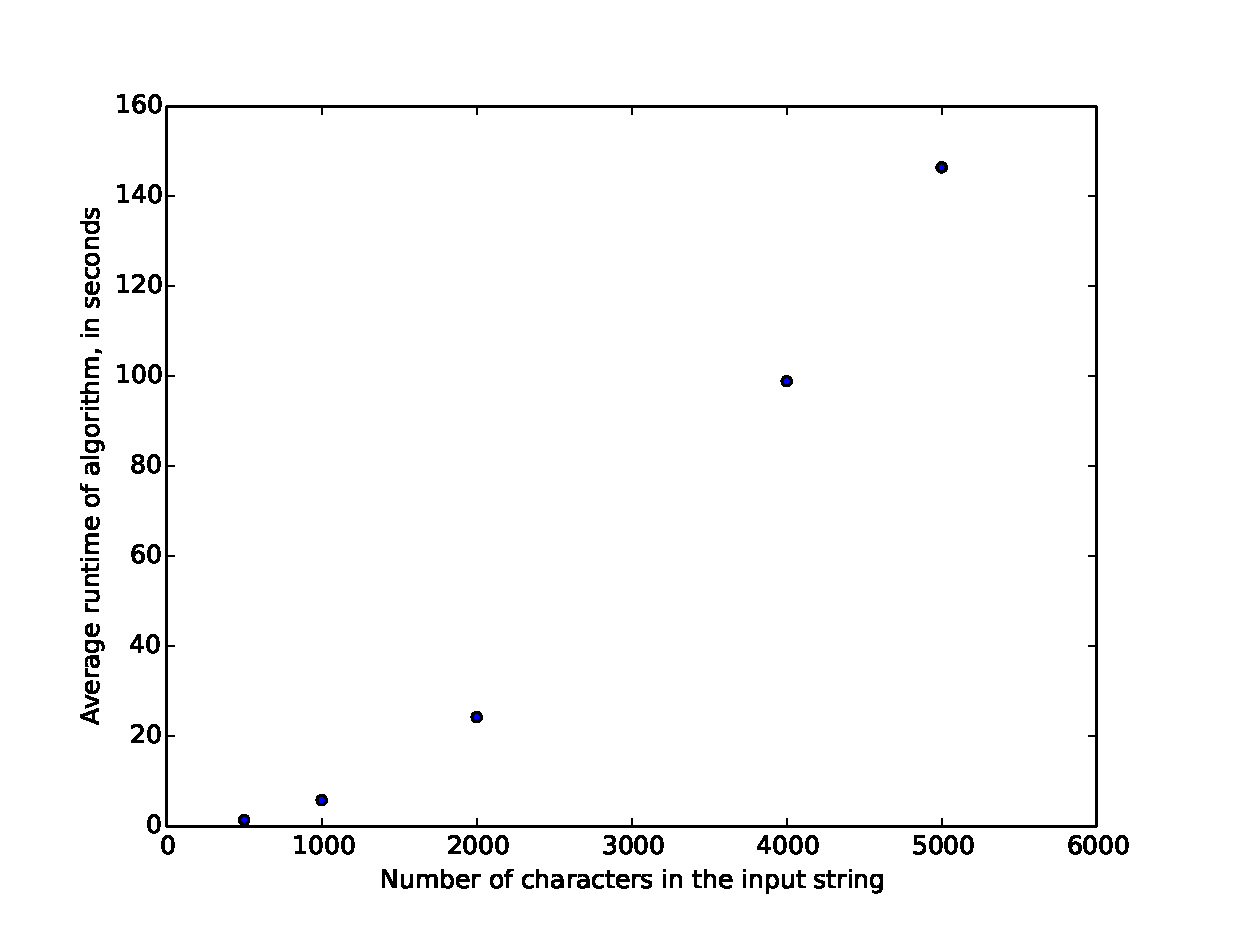
\includegraphics[width=\textwidth]{scatter_graph.eps}
    \caption{Matplotlib.pyplot scatter plot showing the average runtime of the Min Edit Distance Backtrace Alg.}
\end{figure}

\begin{figure}[H]
    \centering
    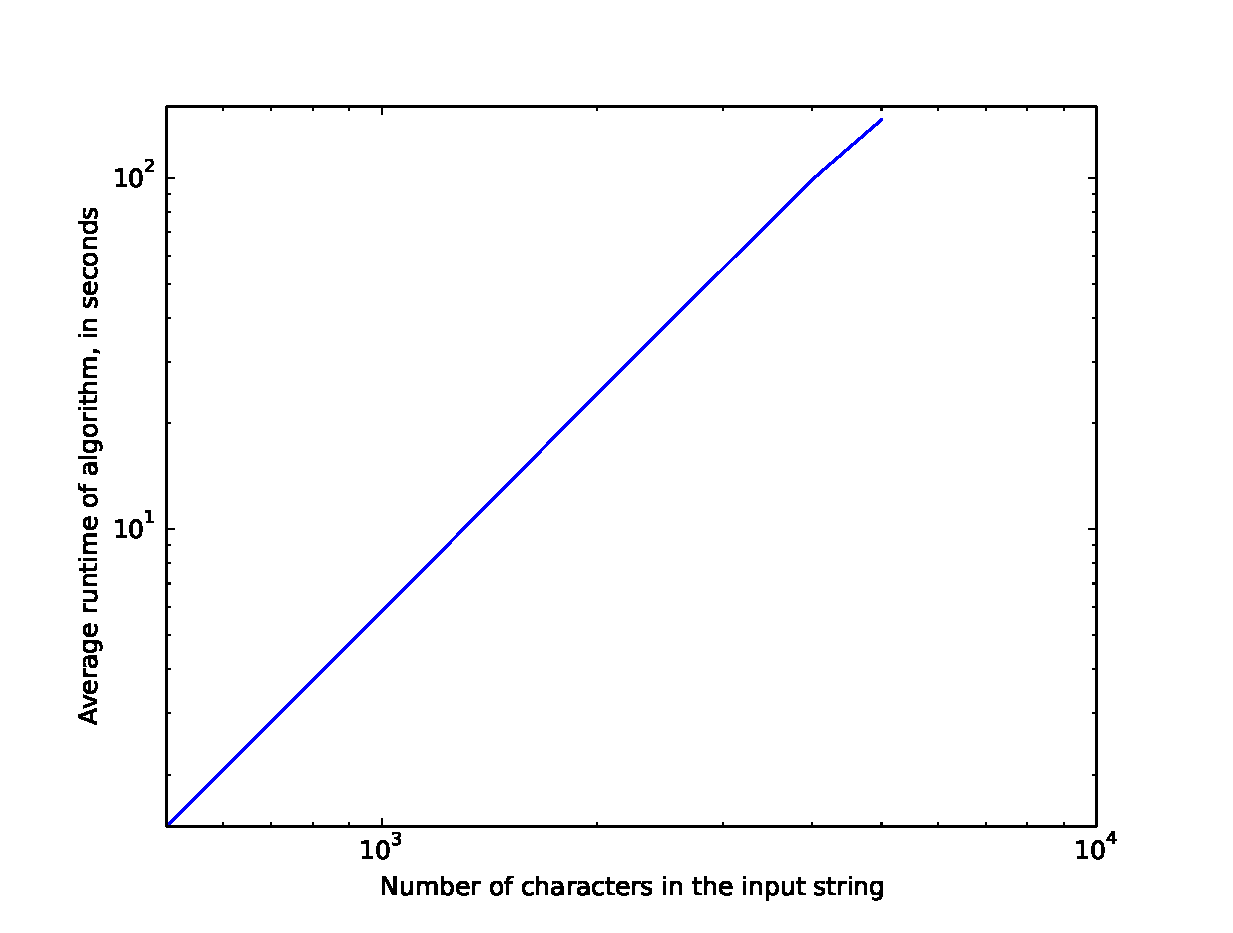
\includegraphics[width=\textwidth]{loglog_graph.eps}
    \caption{Matplotlib.pyplot loglog plot showing the average runtime of the Min Edit Distance Backtrace Alg on a Log-Log scale.
				Using scipy.stats.linregress we found the slope of this line to be m=2.023 with an r-value of .99992.}
\end{figure}

\begin{table}[h]
\centering
	\caption{Comparison of the average runtime in seconds of the Min Edit Distance With Backtrace Algorithm for varying N}
    \begin{tabular}{|p{.15\linewidth}|p{.1\linewidth}|p{.1\linewidth}|p{.1\linewidth}|p{.1\linewidth}|p{.1\linewidth}|}

    \cline{3-3}

    \hline \textbf{Algorithm} & \textbf{N=500} & \textbf{N=1000} & \textbf{N=2000} & \textbf{N=4000} & \textbf{N=5000} \\ \hline

    Min Edit Distance & 1.42413878441 & 5.82820360661 & 24.2761105061 & 98.9141623974 & 146.429415107 \\ \hline

    \end{tabular}
\end{table}

\newpage

The above plots and table were obtained by running the Minimum Edit Distance with
Backtrace implementation on a Samsung Notebook 9 with an Intel CORE i5 processor
and then plotting the resulting runtimes using the Python library: matplotlib.pyplot.
After plotting the runtimes, the scipy.stats.linregress function was applied in order
to calculate the slope of the line in the log-log plot. The code is as follows: \\

\begin{lstlisting}
from scipy.stats import linregress
import numpy as np

times = [   1.42413878441,
        5.82820360661,
        24.2761105061,
        98.9141623974,
        146.429415107 ]

N = [500, 1000, 2000, 4000, 5000]

print linregress(np.log10(N), np.log10(times))

\end{lstlisting}

As mentioned in the caption of Fig.2 this resulted in a slope about 2 and an r-value
extremely close to one. This information leads us to conclude the algorithm has an
experimental runtime of \begin{math}O(N^2)\end{math}.

\newpage

\section{Interpretation and Discussion}

Both of the runtime plots and the linear regression results confirm expectations from
theoretical runtime analysis of the algorithm. The asymptotic analysis indicated
that we would have a runtime of \begin{math}O(MN)\end{math} for the dynamic programming
subroutime and \begin{math}O(M+N)\end{math} for the backtrace. In practice, we
see that \begin{math}O(MN)\end{math} dominates \begin{math}O(M+N)\end{math}. Looking solely
at the linear regression results, \begin{math}O(N^2)\end{math}, and the theoretical
results, \begin{math}O(MN)\end{math}, it appears the results did not match.
However, because the pairs of strings in our experiment were always the same length it turns out that
\begin{math}N^2 = M*N\end{math} and so our results for the theoretical asymptotic
analysis and the empirical analysis match.

\end{document}
